\chapter{Benchmark Results}
\section{Original Version}
\subsection{Java}
\subsection{OCL}
\subsection{EMF-IncQuery}
\subsection{Analysis}


\section{Extended Version}
\subsection{ASE Analysis}
\subsection{Spider Chart}



\concept{Tools} of different technologies were selected to carry out the train
benchmark and compare their efficiency on this model validation task.
All tools are used in a single workstation configuration and accessed in single
user mode. Most tools keep the database in memory (see \figref{table:tools}),
for others RAM disk is created to alleviate the increased time because of disk
access. Common in all tools that they preserve strong consistency. The list of
tools with their version, data description language, query language,
implementation language and incrementality can be found in \figref{table:tools}.

\subsection{EMF tools}
Plain \concept{Java} was choosen as the reference imlementation, although it
does not provide declarative query definition. The benchmark highlights how it
performs compared to the tested tools.

OCL \cite{omg-ocl} is a widely used constraint language, which can be used also
as a query language. \concept{Eclipse OCL} \cite{EclipseOCL} is used to evaluate
these constraints over an EMF metamodel. In the benchmark, the latest code
generation (CG) based approach \cite{ocl-cg} was measured besides the original
implementation.

Incremental OCL query evaluation can be achieved using the \concept{OCL Impact
Analyzer} \cite{ocl-ia} from the Eclipse OCL project. During EMF modifications
it looks for possible context objects that could change the match set, and OCL
re-evaluation can be executed only for those objects. As it is intended only for
incremental use, Eclipse-OCL is used for batch mode. (Batch mode is required for
the benchmark because modifications are based on batch results.)

\todo{UML Analyzer}

\concept{EMF-IncQuery} \cite{models10} is an Eclipse Modeling project that
provides incremental query evaluation using RETE \cite{rete} nets. Queries can
be written in its graph pattern based query language (IncQuery Pattern Language,
IQPL \cite{iqpl}), which is evaluated over EMF models.

Incremental query evaluation is also supported by the \concept{Drools}
\cite{Drools} rule engine developed by Red Hat. It is based on a variant of RETE \cite{rete}
(object-oriented RETE). Queries can be formalized using its own rule description
language. Queries can be constructed by naming the ''when'' part of rules and
acquiring their matches.

%  \concept{Praxis} \cite{praxis} implements an operation-based model checker.
% It translates the instance model and modifications into prolog axioms as a
% series of edit operations. Queries are formalized in SWI-Prolog using the
% provided library.


\begin{table}[Hh]
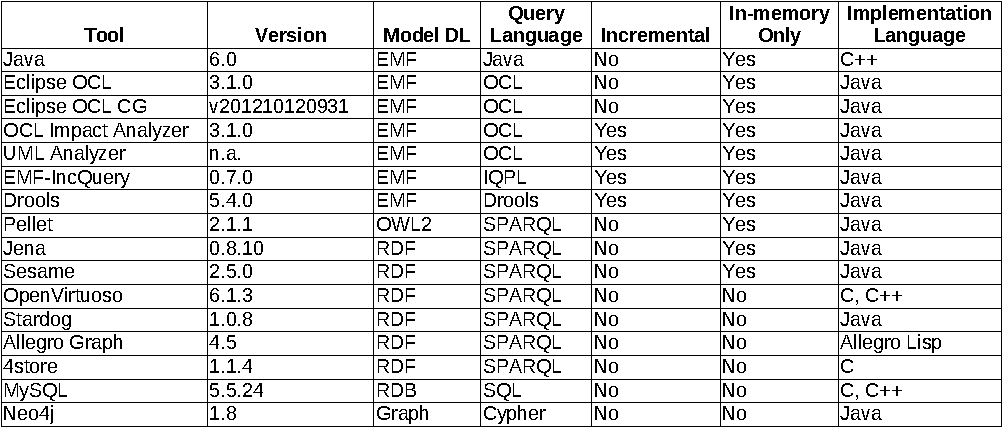
\includegraphics[width=\columnwidth]{figures/tools.pdf}
\caption{Tools used in the benchmark}
\label{table:tools}
\end{table}

\subsection{SPARQL engines}
SPARQL engines are query engines, used to answer graph pattern queries over
ontologies. Basically they perform queries over the raw dataset, but when
(RDF/RDFS or OWL) inferencing is switched on, they can work on the inferred
graph too.

\concept{Pellet} \cite{Pellet} is one of the state of the art reasoners
supporting OWL2 (with direct semantics) and SWRL language reasoning. SPARQL
queries can be executed using the Jena interface. Incremental reasoner is
available, however incremental query engine is not, so it can not be utilized
during the second check.

\concept{Jena} \cite{Jena} defines a standard API for managing RDF or OWL
ontologies, manipulating and querying them. It has a custom in-memory RDF
inferencing engine which is tested.

\concept{Sesame} \cite{sesame} is another widely used API created primarily for
RDF model editing, querying and storing. It has its own RDFS inferencer based on
forward chaining, and part of the inferred model can be retrieved using the
SPARQL language. Note that Open Virtuoso, Stardog and Allegro Graph use this API
with their own storage and query engine implementation.

\concept{Open Virtuoso} \cite{openvirtuoso} is the open source version of the
Virtuoso database engine. It supports unified RDF and RDB storage and SPARQL/SQL
query answering. This engine is widely used as an RDF engine, for example it
backs DBpedia (the RDF version of Wikipedia) and provides public SPARQL access
point to it.

\concept{Stardog} \cite{stardog} is a fast, lightweight, commercial RDF database
for mission-critical apps (as its website describes). It uses SPARQL as query
language, RDF or OWL as model store and Pellet for inferencing.

\concept{Allegro Graph} \cite{allegrograph} is a high performance persistent
graph database. It supports RDFS++ reasoning and SPARQL query answering. It uses
efficient memory utilization in combination with disk-based storage, enabling it
to scale to billions of quads while maintaining superior performance. As other
tools use in-memory backends, the data directory is put into an in-memory
filesystem during the benchmark.

\concept{4store} \cite{harris20094store} is a distributed RDF database, which
can evaluate SPARQL queries. The tool is evaluated in a single machine
environment using the Sesame API. This way, the measuring application is
communicated using the SPARQL protocol with the 4s-httpd, which is connected to
the local 4s-backend. Although distributed query answering is supported, 4store
doesn't offer inferencing because of performance reasons.

\subsection{Relational Databases}
Relational databases are the most widely used technologies for storing and
querying data, even for graph based applications (like OO software). MemSQL is
an in-memory implementation, but it is a rather new technology and for now
doesn't support the necessary subset of SQL to formulate the constraints.
Instead \concept{MySQL} \cite{mysql} was used configured to work as an in-memory
engine. The whole benchmark was adapted to relational databases, without
starting from EMF or using any object-relational mapping technique.

\subsection{Graph Database}
RDF is a graph based structure in itself, but more general graph databases exist
like Neo4j \cite{neo4j}. The data model is based on graphs, where any node or
arc can be labeled. Cypher can be used to query such labeled graphs using its
own graph pattern notation. This engine also uses disk for data storing, so
memdisk is created during the benchmark.

\subsection{Benchmark environment and measurement framework}

In order to measure tool efficiency instead of some bottlenecks (e.g. the lack
of memory) or transient effects (like random CPU hogs), we payed attention to
the hardware-software environment.
The benchmark was executed on a physical machine that contains two quad core
Intel Xeon L5420 CPU ($2.50$~GHz), $32$~GBs of RAM. $64$ bit Ubuntu 12.04 OS
with OpenJDK JVM version 1.6.0\_24 was used. To avoid external influences, such
as swapping, trashing or parallel software execution, swap support, and
unnecessary operating system services (like cron) were turned off, and disk
caches were cleared between executions.
Similarly, to avoid Java \emph{garbage collection}, an extra large heap limit
($15$~GB) was set.

Before acquiring memory usage (free heap space) from the JVM, GC calls were
triggered five times to sweep unfreed objects from the RAM.
The time of each phase was recorded with millisec precision and recorded to CSV
format for later offline evaluation.

To measure the scalability of the tools the implemented queries were executed on
a set of generated models between sizes $30$k and $14$M model elements. Each
total time was limited to $12$ minutes.

To make the performance measurements of a tool for a given query-model pair was
independent from the others, every measurement was run in a different JVM. This
large degree of isolation was required to reduce the effects of complex interference
between queries and instance models.


\subsection{Measurement methodology}
Execution times were recorded using the \emph{java.lang.System.nanoTime()}
function, while memory usage data has been recorded in separate runs using the
\emph{java.lang.Runtime} class. At the tools, where external server is needed
(e.g Open Virtuoso and MySQL) a memory usage of the external process was also
measured using a system call to the OS, that returns the resident set size (RSS)
of the process memory.

To minimize the transient effects of the JVM and OS, that influence the
execution time, all benchmark series was executed ten times and afterwards the
results were noise filtered. We estimated an error model of the measured values:
due to transient effects the measured value everytime increases and never
decreases. We consider the three smallest value of the ten measured values to be
valid measurement results and calculated the average of them. To minimize the
transient effects of Java memory management we execute several garbage collector
invocations before the measurement is done.

TODO: timeout 10 min.

% összes tool

We present the benchmark results in the following two subsections. First, the
global outcome will be shown, where all the tools will take into account.
Afterwards, based on this results the most relevant tools and cases will be
selected and a detailed presentation of our results will be shown.


\section{Original version}
\subsection{Measurement Results}\label{sec:results}

The measurement results of the benchmark is displayed on
\autoref{fig:trainbenchmark-diagrams}. These diagrams show the batch query
performance, incremental evaluation time, and memory usage of each tools, for
different model sizes. Additionally, the initial and the updated result set size
is displayed under the model sizes in the batch and incremental queries,
respectively.

The left column shows charts of the \emph{RouteSensor} query,
while the more complex \emph{SignalNeighbor} is presented in the right column.
The remaining \emph{PosLength} and \emph{SwitchSensor} queries are only presented
at the benchmark website~\cite{TBwebsite}, as their results are very similar to the
\emph{RouteSensor} case.

\subsubsection{Batch Query Evaluation}
In case of batch query evaluation, both OCL implementations use the same
algorithm, thus their execution time is roughly the same. The roughly negligible
differences are due to the initialization of the OCL Impact Analyzer.

For the \emph{batch query} evaluation of the \emph{RouteSensor} query
\autoref{fig:BatchValid_RouteSensor} shows that \incquery{} performs similarly
to Eclipse OCL. It is slightly faster for small models ($2$s and $3$s
respectively), but is slower for large models (up to $125$s and $78$s), where
this $50\%$ slowdown (once in the whole scenario) can be attributed to the
initial (Rete) cache build.

% Both OCL measurements use Eclipse OCL for the batch phase,
% because the Impact Analyser is not built for this purpose according to the
% authors. However, the initialisation of the OCL Impact Analyser also occurs in
% this phase resulting in (roughly negligible) higher execution time.

\begin{figure}[ht]
\begin{center}
	\begin{subfigure}[t]{0.48\textwidth}\centering
	    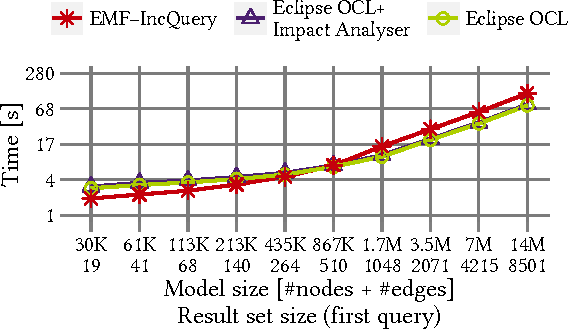
\includegraphics[width=0.9\textwidth]{figures/trainBenchmark_User_BatchValid_RouteSensor}
	    \caption{Batch Query Evaluation Time - RouteSensor}
	    \label{fig:BatchValid_RouteSensor}
	\end{subfigure}
	\begin{subfigure}[t]{0.48\textwidth}\centering
	    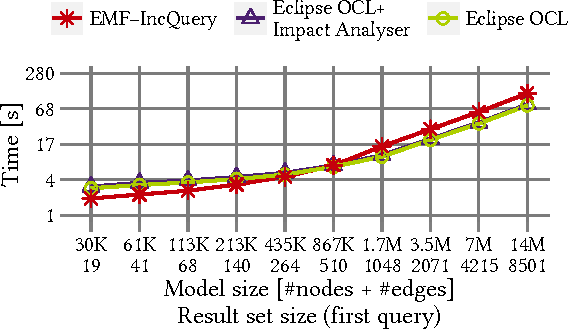
\includegraphics[width=0.9\textwidth]{figures/trainBenchmark_User_BatchValid_RouteSensor}
	    \caption{Batch Query Evaluation Time - SignalNeighbor}
	    \label{fig:BatchValid_SignalNeighbor}
	\end{subfigure} \\

	\begin{subfigure}[t]{0.48\textwidth}\centering
	    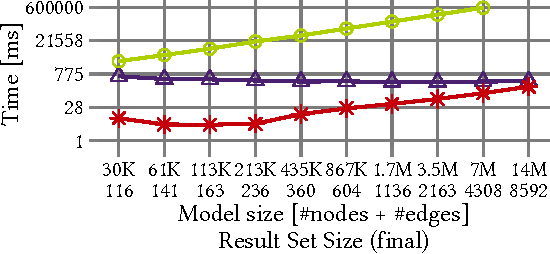
\includegraphics[width=0.9\textwidth]{figures/trainBenchmark_User_SumInc_RouteSensor}
	    \caption{Incremental Query Evaluation Time - RouteSensor}
	    \label{fig:SumInc_RouteSensor}
	\end{subfigure}
	\begin{subfigure}[t]{0.48\textwidth}\centering
	    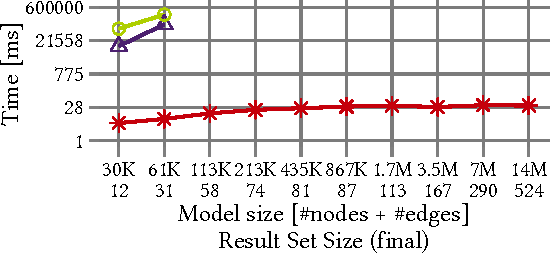
\includegraphics[width=0.9\textwidth]{figures/trainBenchmark_User_SumInc_SignalNeighbor}
	    \caption{Incremental Query Evaluation Time - SignalNeighbor}
	    \label{fig:SumInc_SignalNeighbor}
	\end{subfigure} \\

	\begin{subfigure}[t]{0.48\textwidth}\centering
	    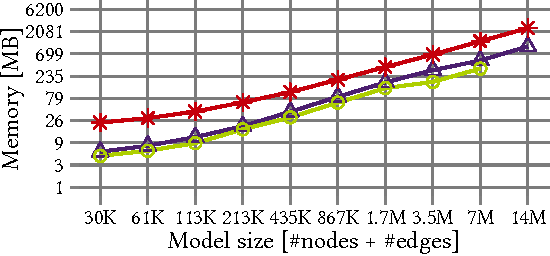
\includegraphics[width=0.9\textwidth]{figures/trainBenchmark_User_Memory_RouteSensor}
	    \caption{Memory Usage - RouteSensor}
	    \label{fig:Memory_RouteSensor}
	\end{subfigure}
	\begin{subfigure}[t]{0.48\textwidth}\centering
	    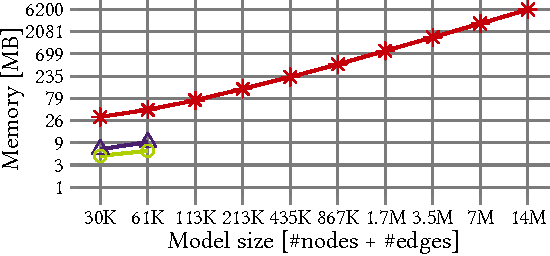
\includegraphics[width=0.9\textwidth]{figures/trainBenchmark_User_Memory_SignalNeighbor}
	    \caption{Memory Usage - SignalNeighbor}
	    \label{fig:Memory_SignalNeighbor}
	\end{subfigure}
  \caption{Benchmark Results}
  \label{fig:trainbenchmark-diagrams}
\end{center}
\end{figure}

For the more complex \emph{SignalNeighbor} query
\autoref{fig:BatchValid_SignalNeighbor} depicts that \incquery{} (somewhat
surprisingly) outperforms OCL solutions: it is noticeably faster for small
modells ($2$s and $4$s), and over $435$k model elements OCL did not finish with
the initial analysis in $12$ minutes. This performance gain might be attributed to
the more efficient (cached) enumeration of instances, and the possibility of
backward navigation (with the help of auxiliary structures) on unidirectional
references used by this query.

\subsubsection{Incremental Query Evaluation}
In the \emph{incremental case}, Eclipse OCL evaluates the query on each issue
(i.e.: hundred times) from scratch, its execution time increases linearly with
model size, resulting slow overall evaluation.

For the \emph{RouteSensor} query (\autoref{fig:SumInc_RouteSensor}), the Impact
Analyzer performs the $100$ modifications in $350$ms regardless of the model
size. On the same query, \incquery{} starts much faster, but its speed reduces
on the larger models (from $9$ to $220$ms). On the other hand, the Impact
Analyzer is an order of magnitude slower on the \emph{SignalNeighbor} query
(\autoref{fig:SumInc_SignalNeighbor}) query: it does not finish in $12$ minutes
for models over $61$k model elements, while \incquery{} handles every model
regardless of size under $40$ms.

The performance of the Impact Analyzer is most likely affected by the previously
mentioned unidirectional references. The slowdown of \incquery{} is probably
caused by the increased number of matches (from $116$ to $8592$), as query
results are always available in the output nodes of Rete networks, and only a
linear traversal of these stored matches is needed to return them.

% is much faster, moreover performs its task in constant time.
% \incquery{} is faster than OCL Impact Analyser, but it somewhat increases for
% larger $x$ values. The evaluation time of the Rete based \incquery{} does not
% depend on model size, but on the notifications and result set size of output
% nodes (see \autoref{fig:incquery-rt-arch}). As in this testcase modifications
% are similar, this slight increase can be attributed to the change of the number
% of results from 141 to 8592. When the result sets does not vary much, it can
% return query results almost in constant time (be it a small or very large model)
% that is confirmed by \autoref{fig:SumInc_SignalNeighbor}. On the other hand,
% Eclipse OCL slows down and shows linear characteristics (as it is not an
% incremental solution), but interestingly, OCL Impact Analyzer behaves similarly.
% The Impact Analyzer is also orders of magnitude slower and the query evaluation
% time linearly increases as model size increases, perhaps due to the properties
% of the query described in the previous paragraph. In this case the OCL tests
% could be run only for the two smallest model, because for larger models the
% batch and incremental phases took in more than ten minutes resulting in timeout.

